\documentclass[a4paper,12pt]{article}
\usepackage{geometry}

% Set small borders with the geometry package
\geometry{
  top=2cm,     % Top margin
  bottom=2cm,  % Bottom margin
  left=2.5cm,    % Left margin
  right=2.5cm,   % Right margin
}

\usepackage{amsmath}  % For mathematical symbols and equations
\usepackage{amsfonts} % For extra fonts
\usepackage{graphicx} % For including graphics
\usepackage{hyperref} % For hyperlinks (optional)
\usepackage{subcaption}
\usepackage{siunitx}
\usepackage{here}
\usepackage[
    backend=biber,
    sorting=none,
]{biblatex}
\addbibresource{references.bib}

\usepackage{setspace} % For line spacing
% \onehalfspacing


\title{Wave Optical Simulation of Thick Optical Elements}
\author{Felix Wechsler\footnote{École Polytechnique Fédérale de Lausanne (EPFL), Switzerland, \url{felixwechsler.science}}}
\date{\today}
\setlength\parindent{0pt}
\begin{document}
\maketitle
\thispagestyle{empty}

\begin{abstract}
In this article, we outline our approach on simulating optical lenses using a wave optics framework. 
We aim to apply and compare various methods for accurately modeling wave propagation through a thick lens, evaluating each method's performance.
\end{abstract}


\section{Introduction}
Ray optical tools are standard tools to characterize optical elements. However, working on smaller scales the wave nature of light is not negligible.
In this work, we study if simple wave optical algorithms such as the angular spectrum method of plane waves (AS) are suitable to
simulate thick optical elements.
In a concrete example of a spherical lens, we demonstrate how the multi-slice angular spectrum method fails to predict geometrical parameters such as the focal length correctly.
We explore how more advanced methods such as the modified wave propagation method \cite{schmidt2016wave} are able to predict those properties at an 
acceptable computational complexity. 


\section{Theoretical basis}
This section introduces briefly the main concepts behind the different approaches.
For more details, please see the listed references.
\subsection{Angular spectrum method of plane waves}
The angular spectrum method of plane waves (AS) is a solution to the homogenous, isotropic Helmholtz equation which describes free space wave propagation
in a medium with constant and isotropic refractive index $n$.
The mathematical form is
\begin{align}
\psi_{z}&=\mathcal{F}^{-1}\left[\mathcal{F}\left[\psi_{0}\right] \cdot H_{\textrm{AS}}\right],\\
H_{\textrm{AS}}\left(f_{x},f_{y}\right)&=\exp\left(i2\pi z\sqrt{\frac{n^2}{\lambda^{2}}-f_{x}^{2}-f_{y}^{2}}\right)
\end{align}
where $\psi_0$ is the incoming scalar electrical field, $\mathcal{F}$ the 2D Fourier transform, $\lambda$ the wavelength in vacuum, $z$ the propagation distance and $f_{x/y}$ the spatial frequencies in Fourier domain.
Computationally, this can be implemented with two Fast Fourier transform (FFT) algorithms albeit circular wrap-around artifacts of the FFT should be avoided
with the band-limited version of the AS \cite{matsushima2009band}.


\subsection{Multi-slice}
Multi-slice propagation (MS) is an approach to solve wave-propagation in an inhomogeneous (spatially varying refractive index) medium. 
The angular-spectrum method can be extended to multi-slice propagation by dividing the medium into small slices along the optical axis and applying the angular spectrum method to each slice \cite{https://doi.org/10.1107/S0365110X57002194,Li_Wojcik_Jacobsen_2017}. Between each slice, the effect of the medium is 
described as a \textit{thin medium} which allows to include the effect of the medium as a phase shift to the electrical field.
For example, propagation through a medium $n(x,y,z)$ can be described as a series of $N_z$ AS steps $\mathcal{A}$ which corresponding phase shift in between.
The total propagation distance $z$ is split into $\Delta z = z / N_z$ steps.
$n_0$ is an average refractive index of the medium and $k_0$ is the wavenumber in this medium $n_0$. It can be written as
\begin{align}
    \psi(x,y,z) = \underbrace{\mathcal{A}\bigg[\exp\left(i k_0 n(x,y, N_z \cdot \Delta z)\mathcal{A}\big[\exp\left(i k_0 n(x,y, (N_z - 1) \cdot \Delta z) \right) \cdots \psi(x,y, 0) \big] \right) \bigg]}_{N_z \text{ times application of }\mathcal{A}}. 
\end{align}
In \autoref{sec:sim} we show that this method fails to predict geometrical properties of thick optical elements.
The reason is, that if the mediums refractive index deviates from $n$, the MS applies only phase shifts to the electrical field which neglects the actual wavelength change.
Let us do the following Gedankenexperiment that $n_0 = 1$ but the medium in fact has a constant refractive index of $n=1.5$. If we would
propagate a Gaussian beam through this medium, MS would only do constant phase shifts since $n$ is constant at all $(x,y,z)$. But, a constant phase shift will not change any curvature of the beam. But, the curvature change of a Gaussian beam depends on the refractive index the beam is propagating through. It can be seen as if the MS is doing a correct phase change but it is not changing the wavelength accordingly. 

\subsubsection{Modified wave propagation method}
To overcome the shortcomings of the MS, the modified wave propagation method (MWPM) was proposed \cite{schmidt2016wave}.

In integral form, the wave propagation can be written as
\begin{align}
\label{wpm}
    \psi(x,y,z+\Delta z) &= \frac{1}{2\pi} \int \widetilde{\psi}(k_x, k_y, z) \, e^{ik_z(k_x, k_y, x, y) \Delta z} \, e^{i (k_x x + k_y y)} \, \mathrm{d}k_x \, \mathrm{d}k_y\\
    k_z(k_x, k_y, x, y) &= \sqrt{k_0^2 n^2 \left( x,y,z + \frac{\Delta z}{2} \right) - k_x^2 - k_y^2}
\end{align}
where $\widetilde{\psi}$ is the Fourier transform of the electrical field $\psi$.
The spatially varying $k_z(k_x, k_y, x, y)$ forbids to express \autoref{wpm} as a Fourier transform integral.
However, the MWPM argues to express this integral as a sum of piecewise constant functions which are stitched together at regions where $n$ changes.
This assumes there is a finite number of regions where $n$ suddenly changes such as in the case of air and lens interfaces.
\begin{align}
    I_m^z(x,y) &=
    \begin{cases}
    1 & n_z(x,y) = n_m, \\
    0 & n_z(x,y) \ne n_m,
    \end{cases}, \\
    \psi(x,y,z+\Delta z) &= \sum_m I_m^z(x,y) \mathcal{F}^{-1} \left\{ e^{i k_z^m(k_x,k_y)\Delta z} \mathcal{F} \left\{\psi(x,y,z) \right\} \right\},\\
    k_z^m(k_x, k_y) &= \sqrt{k_0^2 n_m^2 - k_x^2 - k_y^2} + \kappa(k_x, k_y).
\end{align}
$k_z^m$ is the wavenumber in the medium $m$.
The MWPM can be implemented with one MS step for each medium $m$.
Qualitatively, it resolves the issue of the MS to not use the correct diffraction kernel of the respective medium. If the medium is piecewise constant, the MWPM can be applied to the cost of one AS step for each medium.

\subsubsection{Hankel transform based methods}
As the last concept we introduce a Hankel transform based wave propagation \cite{Guizar-Sicairos_Gutiérrez-Vega_2004}.
The Hankel transform is a generalization of the Fourier transform to cylindrical coordinates. It can be used to describe the propagation of a wave through a medium with cylindrical symmetry such as a spherical lens.

Let us recall that the Fourier transform can be written as

\begin{equation}
\mathcal{F}[f](k_x, k_y) = \int_{-\infty}^{\infty} f(x,y) \exp(i (k_x \cdot x + k_y \cdot y)) \,\mathrm{d}x\, \mathrm{d}y = \int_{-\infty}^{\infty} f(x,y) \exp(i \vec k \cdot \vec r) \,\mathrm{d}x\, \mathrm{d}y
\end{equation}
If we transform this to polar coordinates $(r, \theta)$ and $(\kappa, \phi)$ we obtain
\begin{equation}
\mathcal{F}[f](\kappa, \phi) = \int_{0}^{\infty} \int_{0}^{2\pi} r f(r, \theta)\cdot \exp(i \cdot \cos(\theta - \phi) \kappa r)  \,\mathrm{d}\theta\, \mathrm{d}r
\end{equation}
where $\kappa = \sqrt{k_x^2 + k_y^2}$ and $r=\sqrt{x^2 + y^2}$

We can now use
\begin{equation}
\exp(i x \cdot \sin(\theta)) = \sum_{n=-\infty}^{\infty} J_n(x) \cdot \exp(i n \theta)
\end{equation}
where $J_n$ is the nth-order Bessel function of the first kind.

After integration (if $f$ has no $\theta$ dependency) over $\theta$ it only remains

\begin{equation}
\mathcal{F}[f](\kappa, \phi) = 2\pi \int_{0}^{\infty} r \cdot f(r) \cdot J_0(\kappa \cdot r) \, \mathrm{d}r = \mathcal{H}[f](\rho)
\end{equation}
where $\mathcal{H}$ is the Hankel transform.
With the Fast Hankel transform \cite{Guizar-Sicairos_Gutiérrez-Vega_2004} we can now efficiently calculate the 2D field propagation with a 1D matrix-vector-product. If required, the radial 1D field can be reconverted to cartesian coordinates. 

\section{Simulation Results}
\label{sec:sim}
In this part, we present our main results of the simulation study. For all details of the simulation, please see the supplemental source code\footnote{\url{github.com/roflmaostc/Wave_Optics_Propagation_Through_A_Lens/}}.
In all three figures in this section, we show the propagated intensity of the incoming Gaussian beam of waist radius \SI{15}{\micro\meter} and $\lambda=\SI{633}{\nano\meter}$. The images are shown with a gamma factor of $0.2$ to increase visibility of low intensity regimes. The green lines always indicate the physical location of a glass ball with refractive index of $1.5$ which is embedded in air with $n=1$.
Also, we distinguish between \textit{hard lens} and \textit{smooth lens}. The first one is a binary discretization of the refractive index array with either 1 or 1.5. The latter is a smooth discretization of the lens where voxels on the boundary have the weighted sum of $n=1$ and $n=1.5$ according to the volume of this voxel being inside of the lens.

\subsection{Multi-slice propagation}
As we see in \autoref{fig:MS}, the MS is able to focus the light. However, the yellow line indicates the focal length of the ball lens derived with the thick lensmaker equation. There is a significant deviation from the simulated and the real focal length. A similar effect has been observed in literature too \cite{schmidt2016wave} though their matrix based beam propagation method overestimates the focal length.
\begin{figure}[H]
    \centering
    \begin{subfigure}[]{0.5\textwidth}
        \centering
        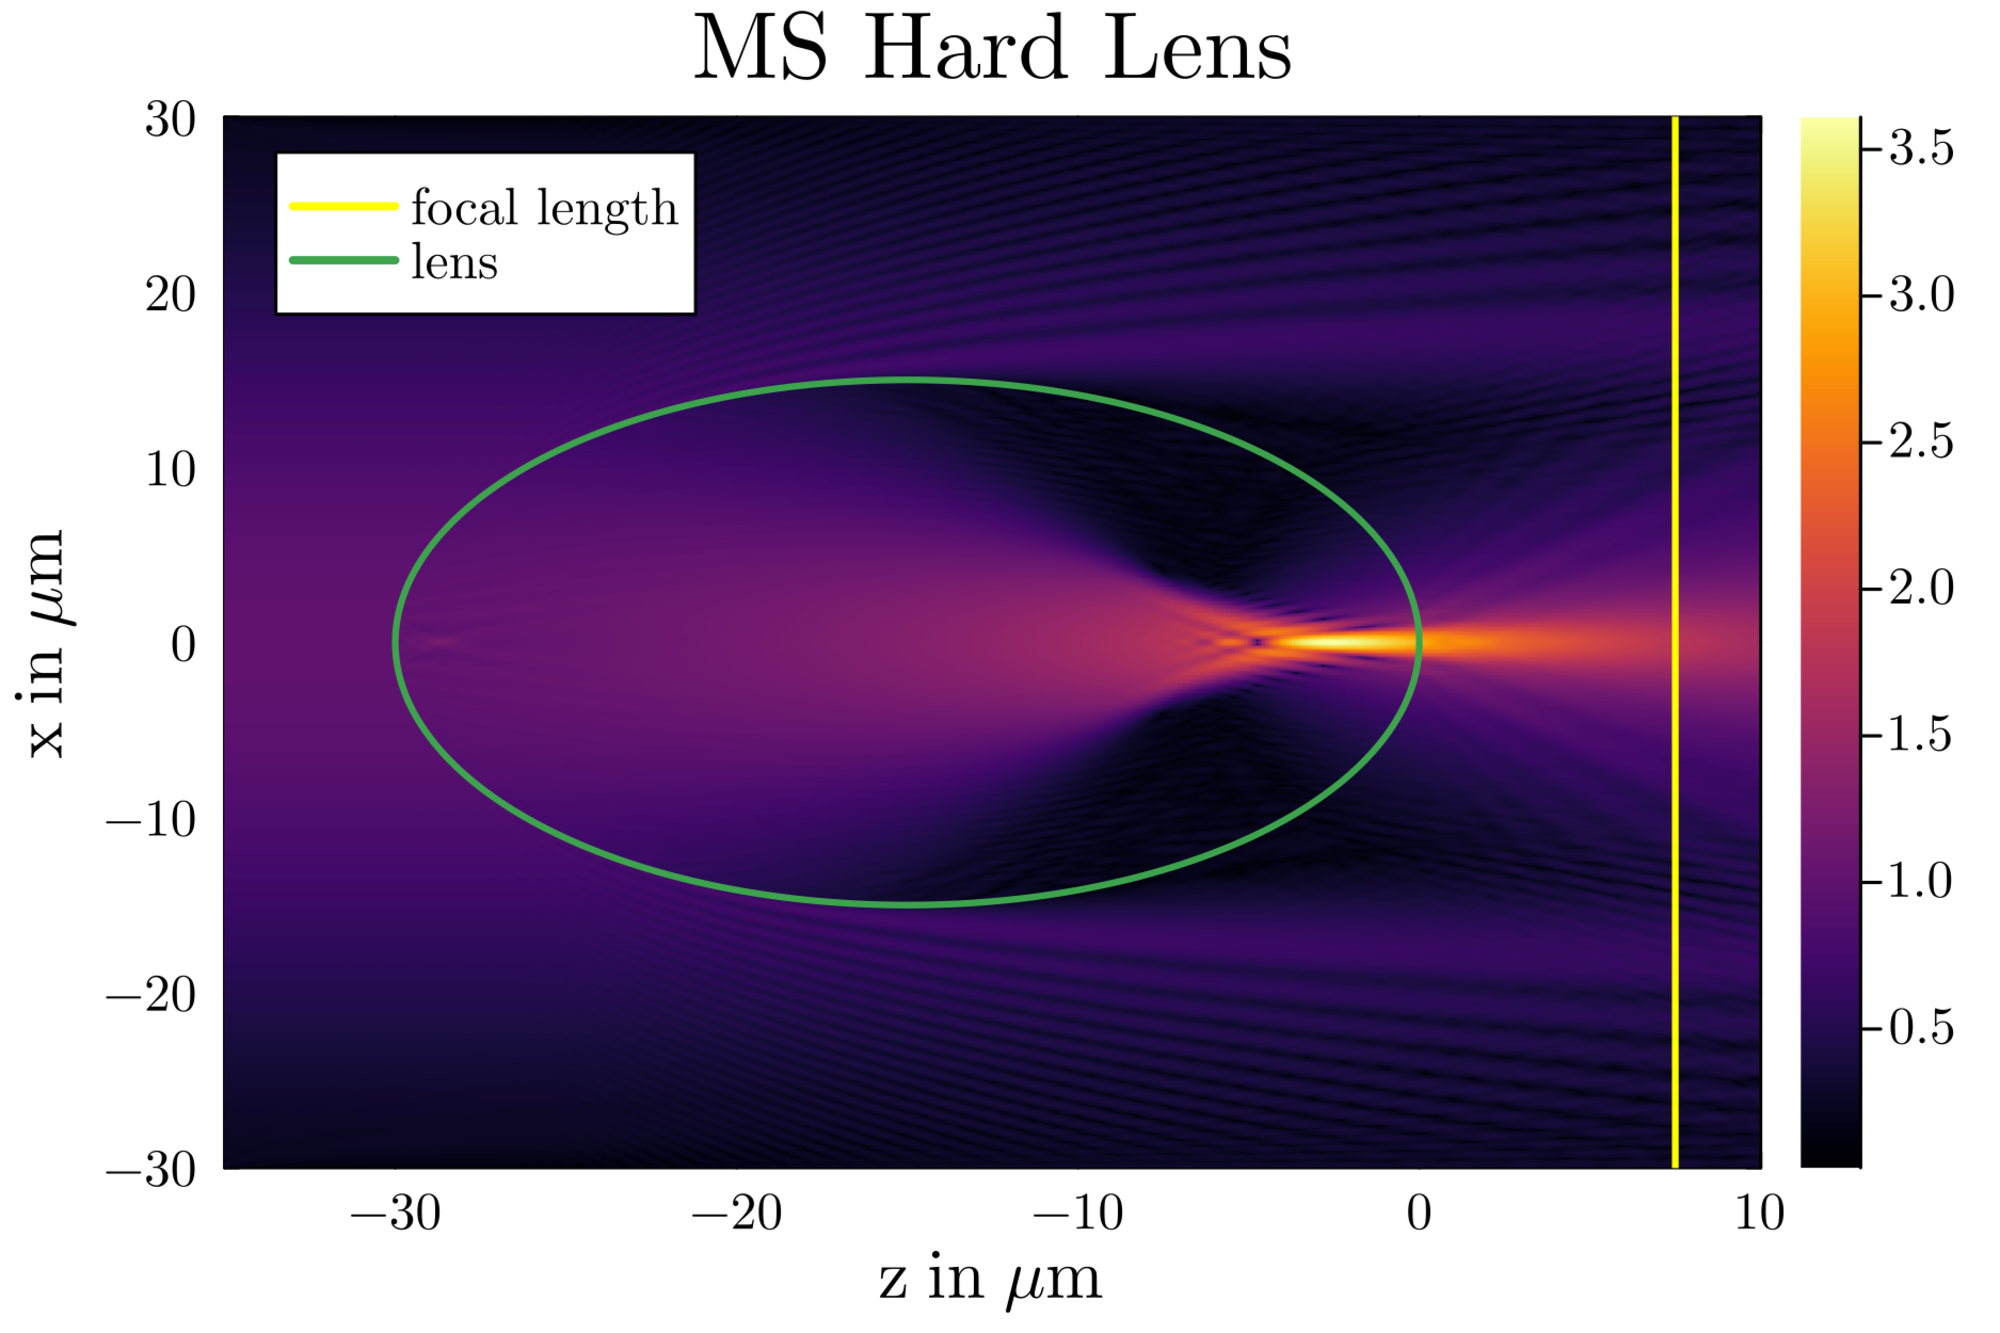
\includegraphics[width=\textwidth]{../figures/MS_hard.svg.png} 
    \end{subfigure}%
    \begin{subfigure}[]{0.5\textwidth}
        \centering
        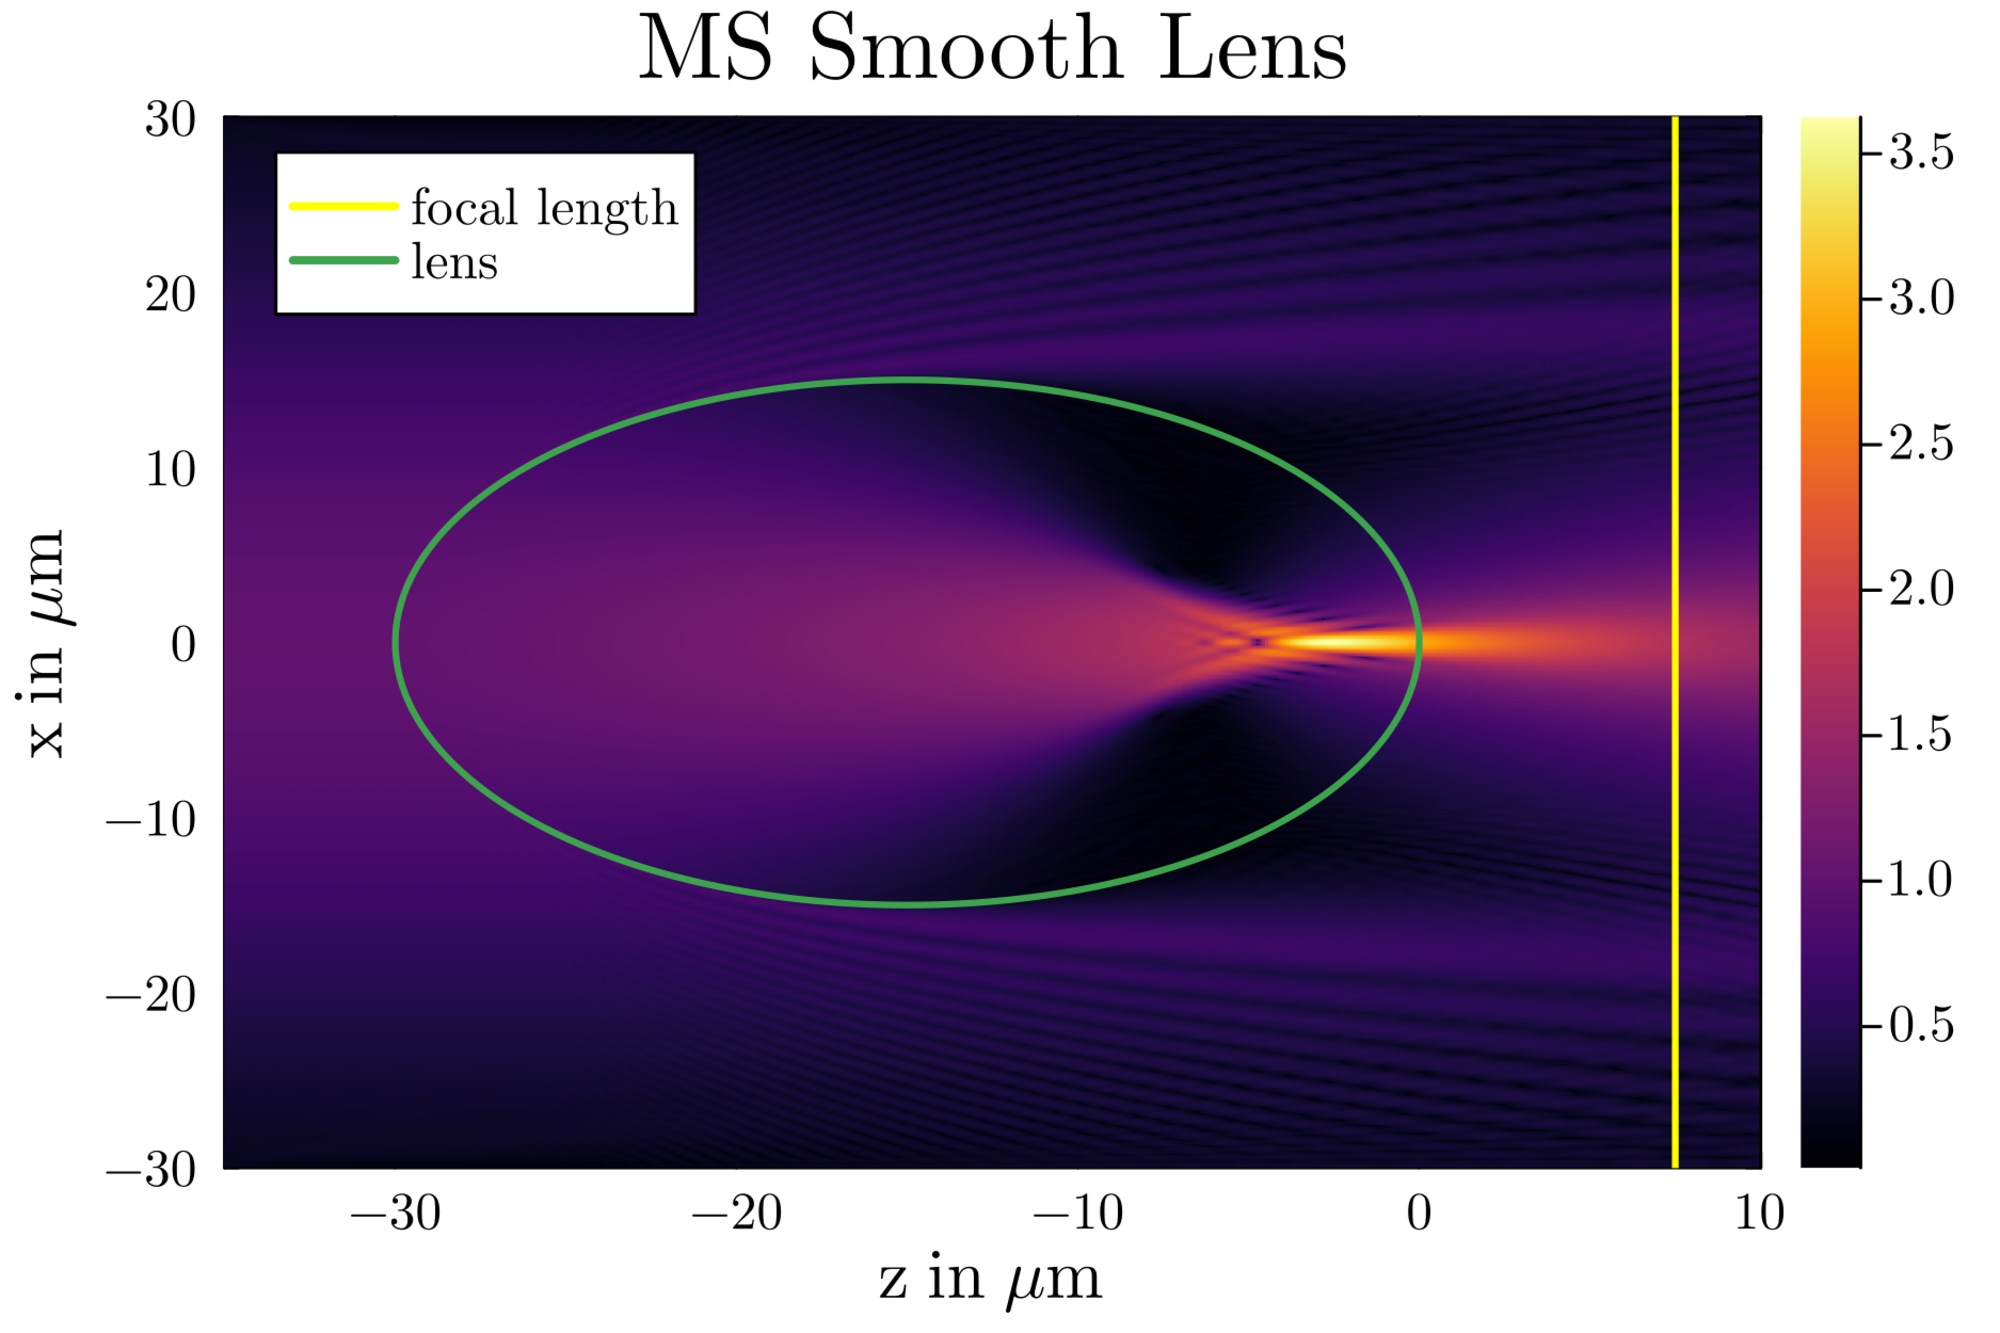
\includegraphics[width=\textwidth]{../figures/MS_soft.svg.png} 
    \end{subfigure}
    \caption{Results of the MS simulation.}
    \label{fig:MS}
\end{figure}
We believe the underestimation stems from the aforementioned mistake of the MS that the propagation kernel inside the glass medium is systematically wrong. The MS applies correct phase shifts but it neglects the $\lambda$ is also changing in that medium.
Also, we see that the smooth lens discretization removes some minor artefacts which are visible at the entrance of the lens at around $z=\SI{-30}{\micro\meter}$.
The number of samples is $N_{x,y} = 1024$ and $N_z=512$. On a Intel Core Ultra 7 155U with Julia 1.11 the simulation took around \SI{200}{\second}.

\subsection{Modified wave propagation method}
The MWPM as proposed by \cite{schmidt2016wave} produces matching results for the focal length. If we use the smooth lens discretization we obtain a very \textit{good looking} intensity without obvious artefacts.
\begin{figure}[H]
    \centering
    \begin{subfigure}[]{0.5\textwidth}
        \centering
        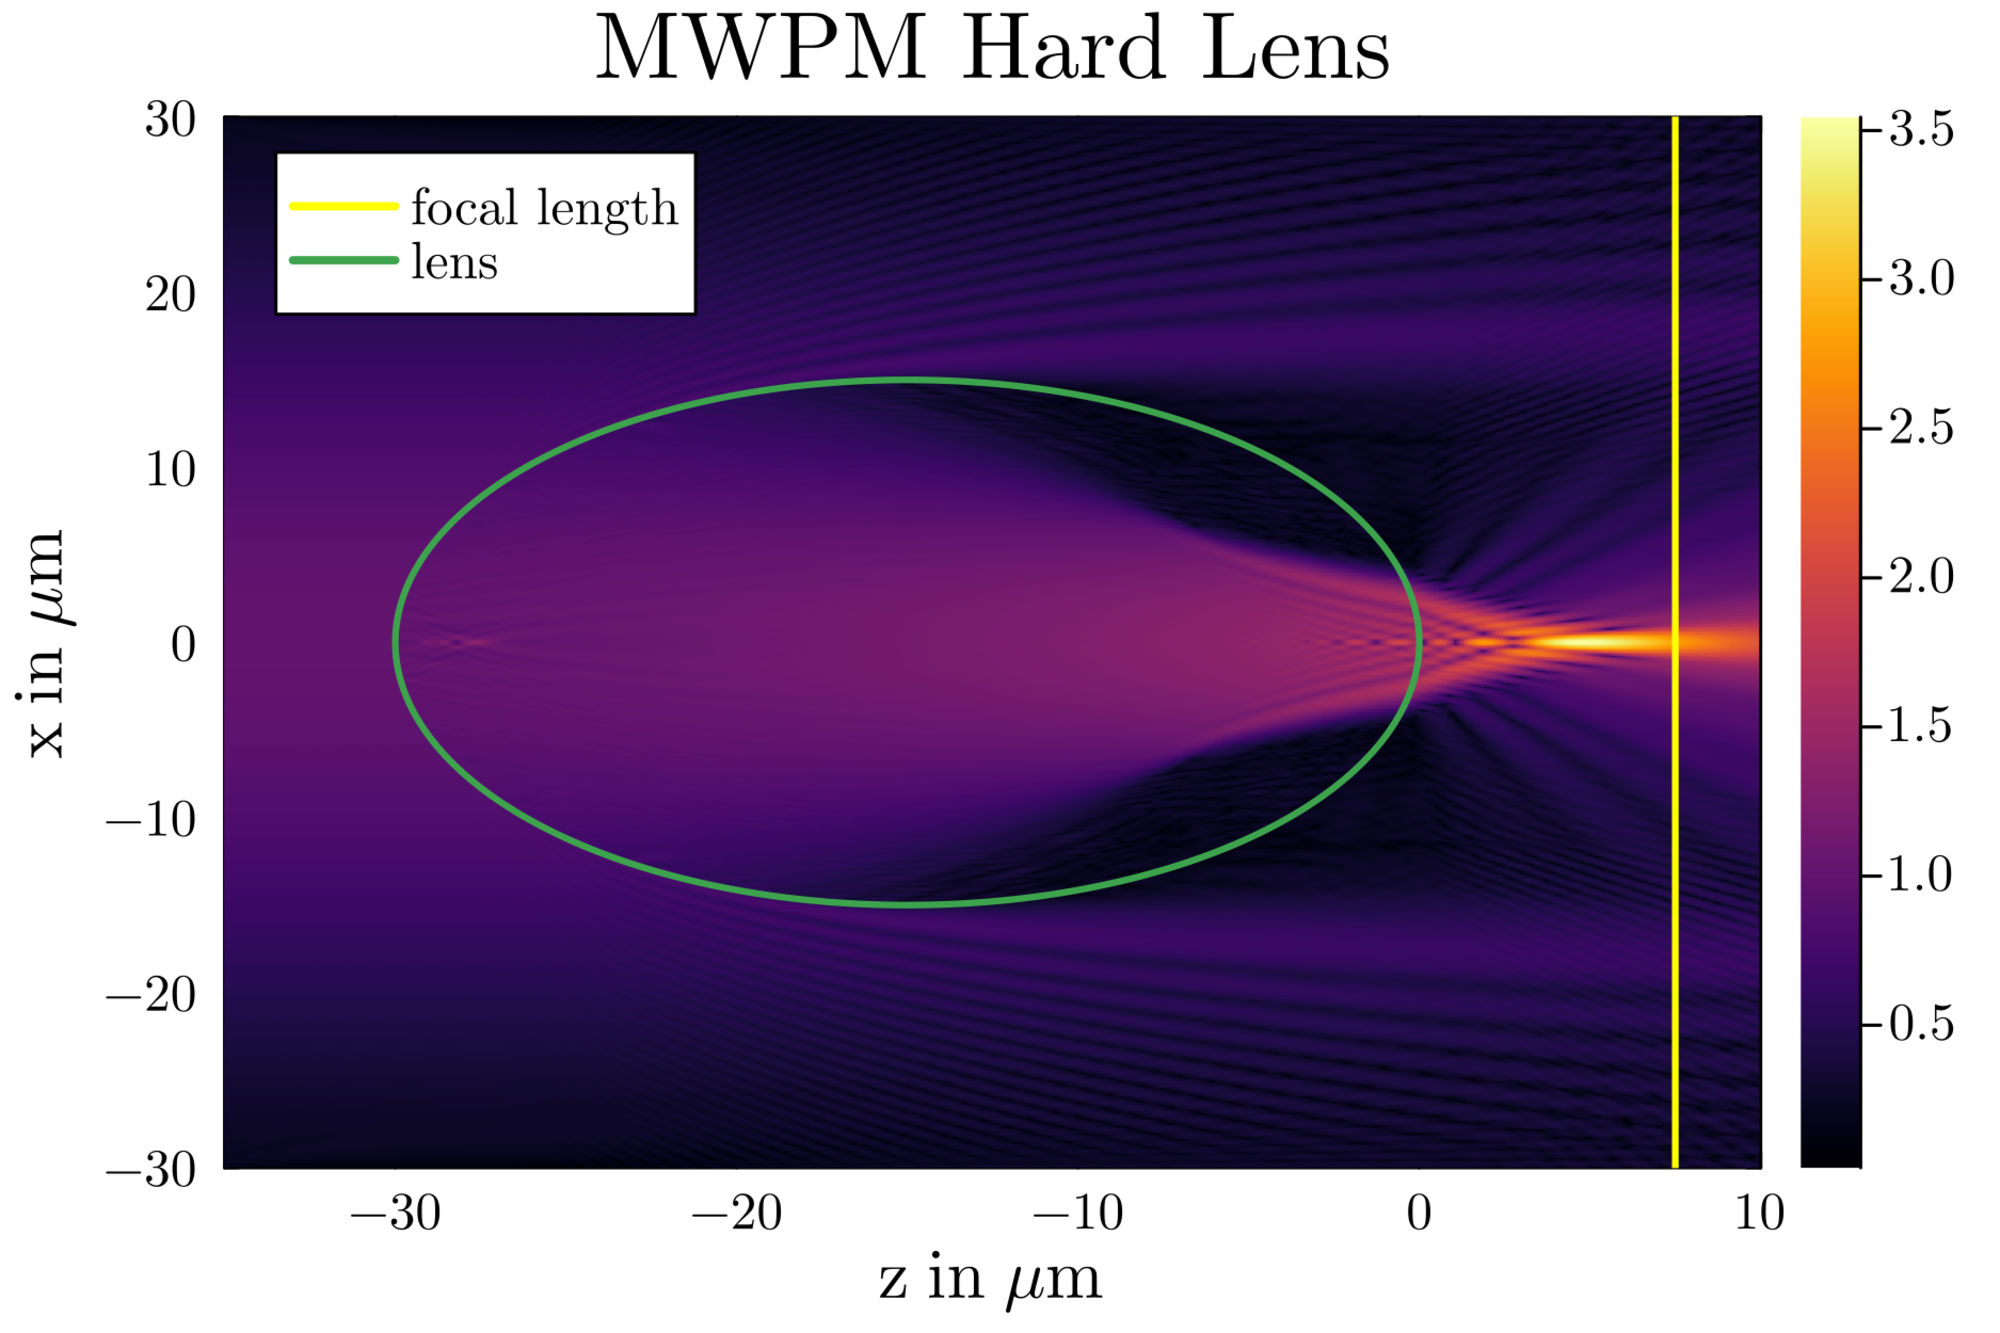
\includegraphics[width=\textwidth]{../figures/MWPM_hard.svg.png} 
    \end{subfigure}%
    \begin{subfigure}[]{0.5\textwidth}
        \centering
        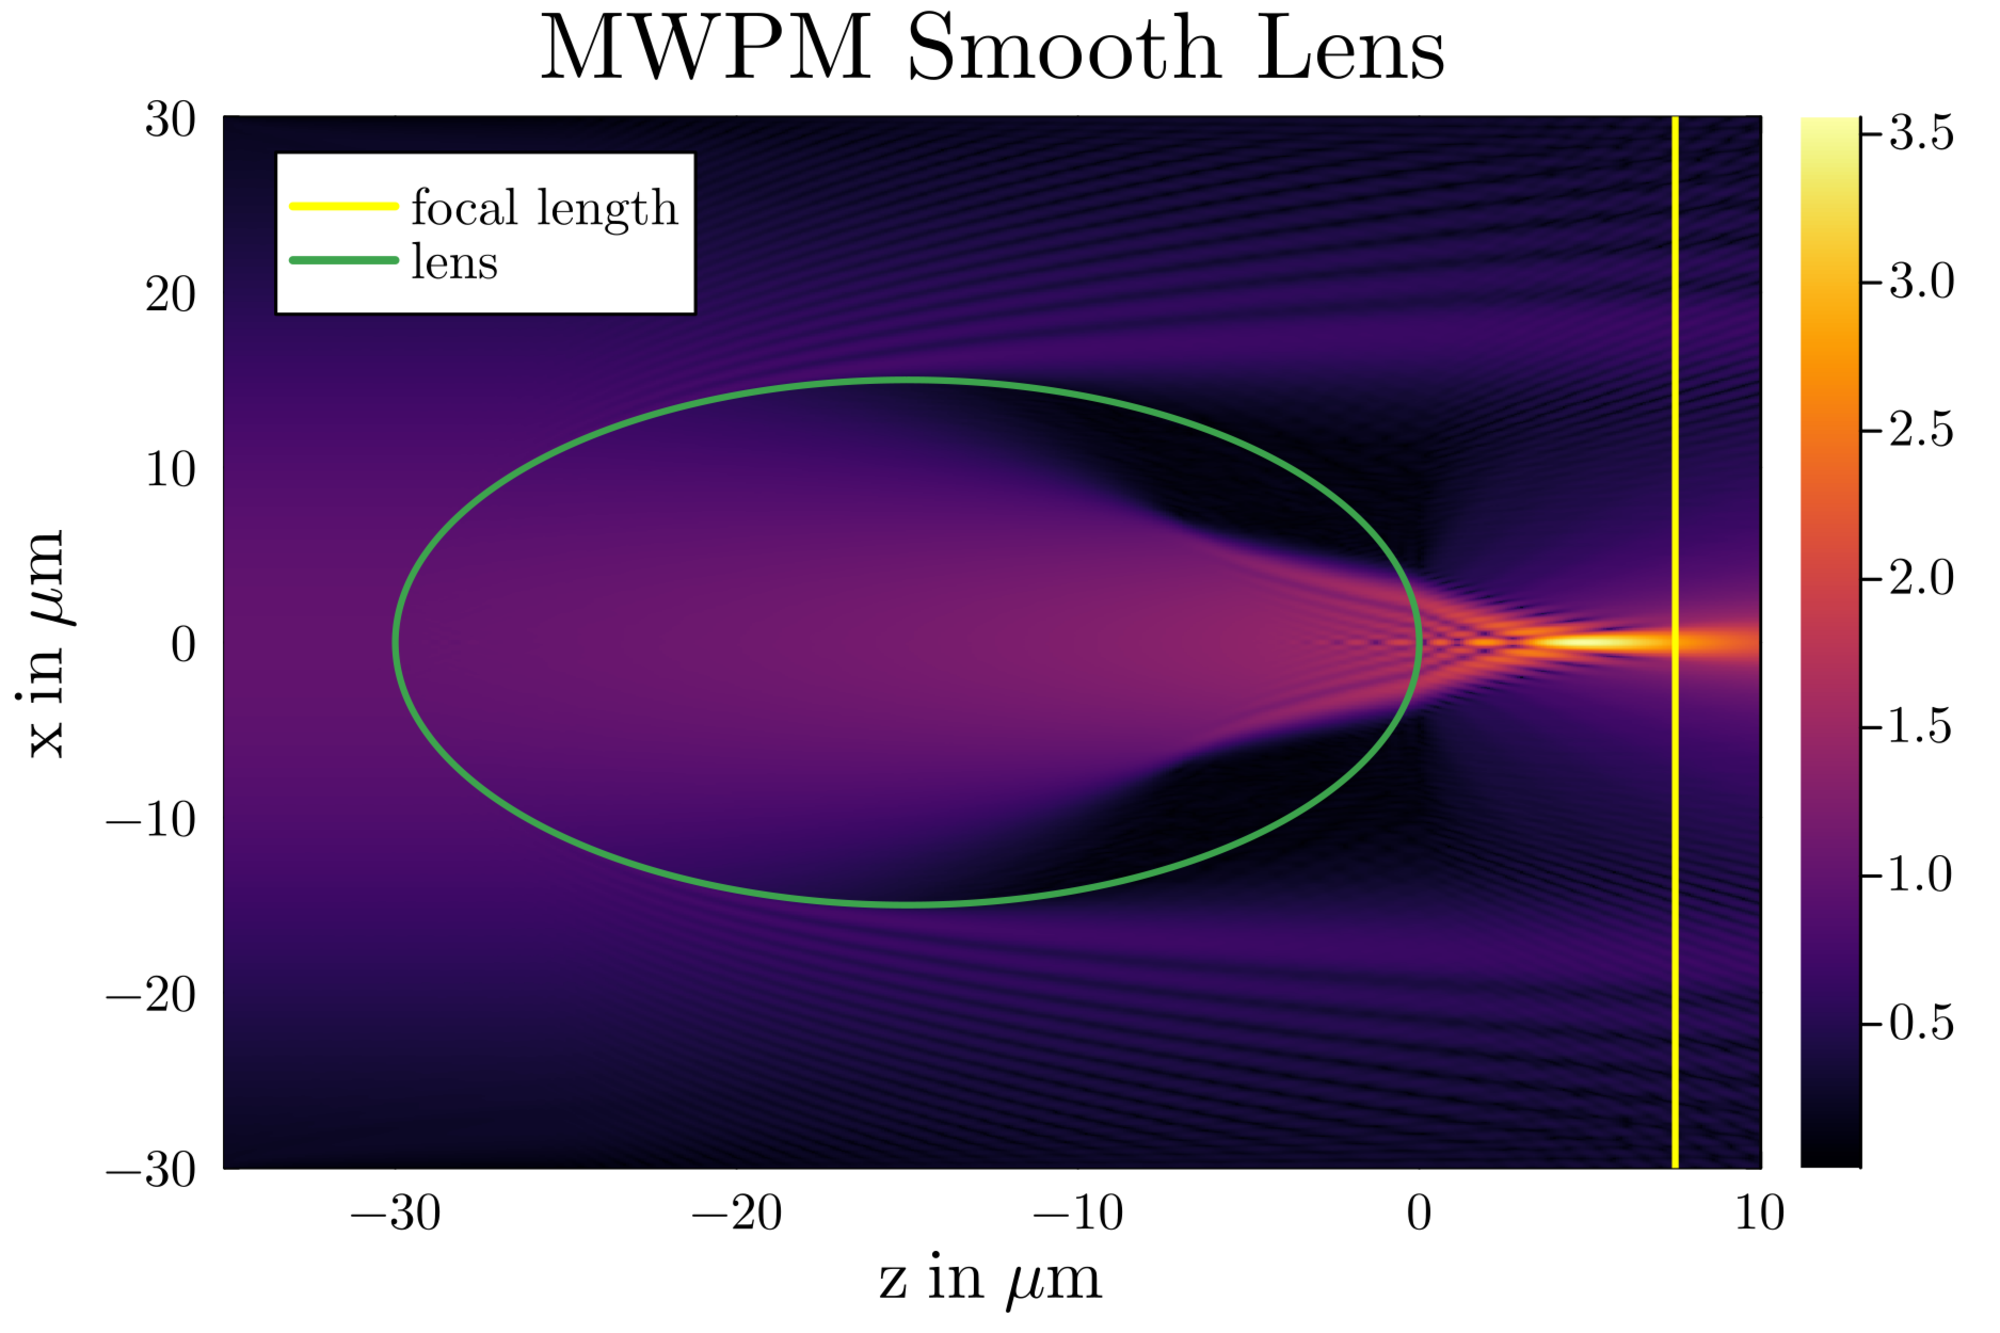
\includegraphics[width=\textwidth]{../figures/MWPM_soft.svg.png} 
    \end{subfigure}
    \caption{Results of the MWPM simulation.}
    \label{fig:}
\end{figure}
This matches well with rigorous solutions of Maxwell's equation in literature. 

\subsection{Hankel transform based methods}
As the Hankel transform method is mathematically identical to the FFT based method for a circular symmetric case, the results are visually identical.
However, due to the reduced computational load (from the 2D to 1D reduction), we can simulate $N_{x,y} = 2048$ and $N_z=1024$ at a faster calculation time of only $\SI{7}{\second}$. 
\begin{figure}[H]
    \centering
    \begin{subfigure}[]{0.5\textwidth}
        \centering
        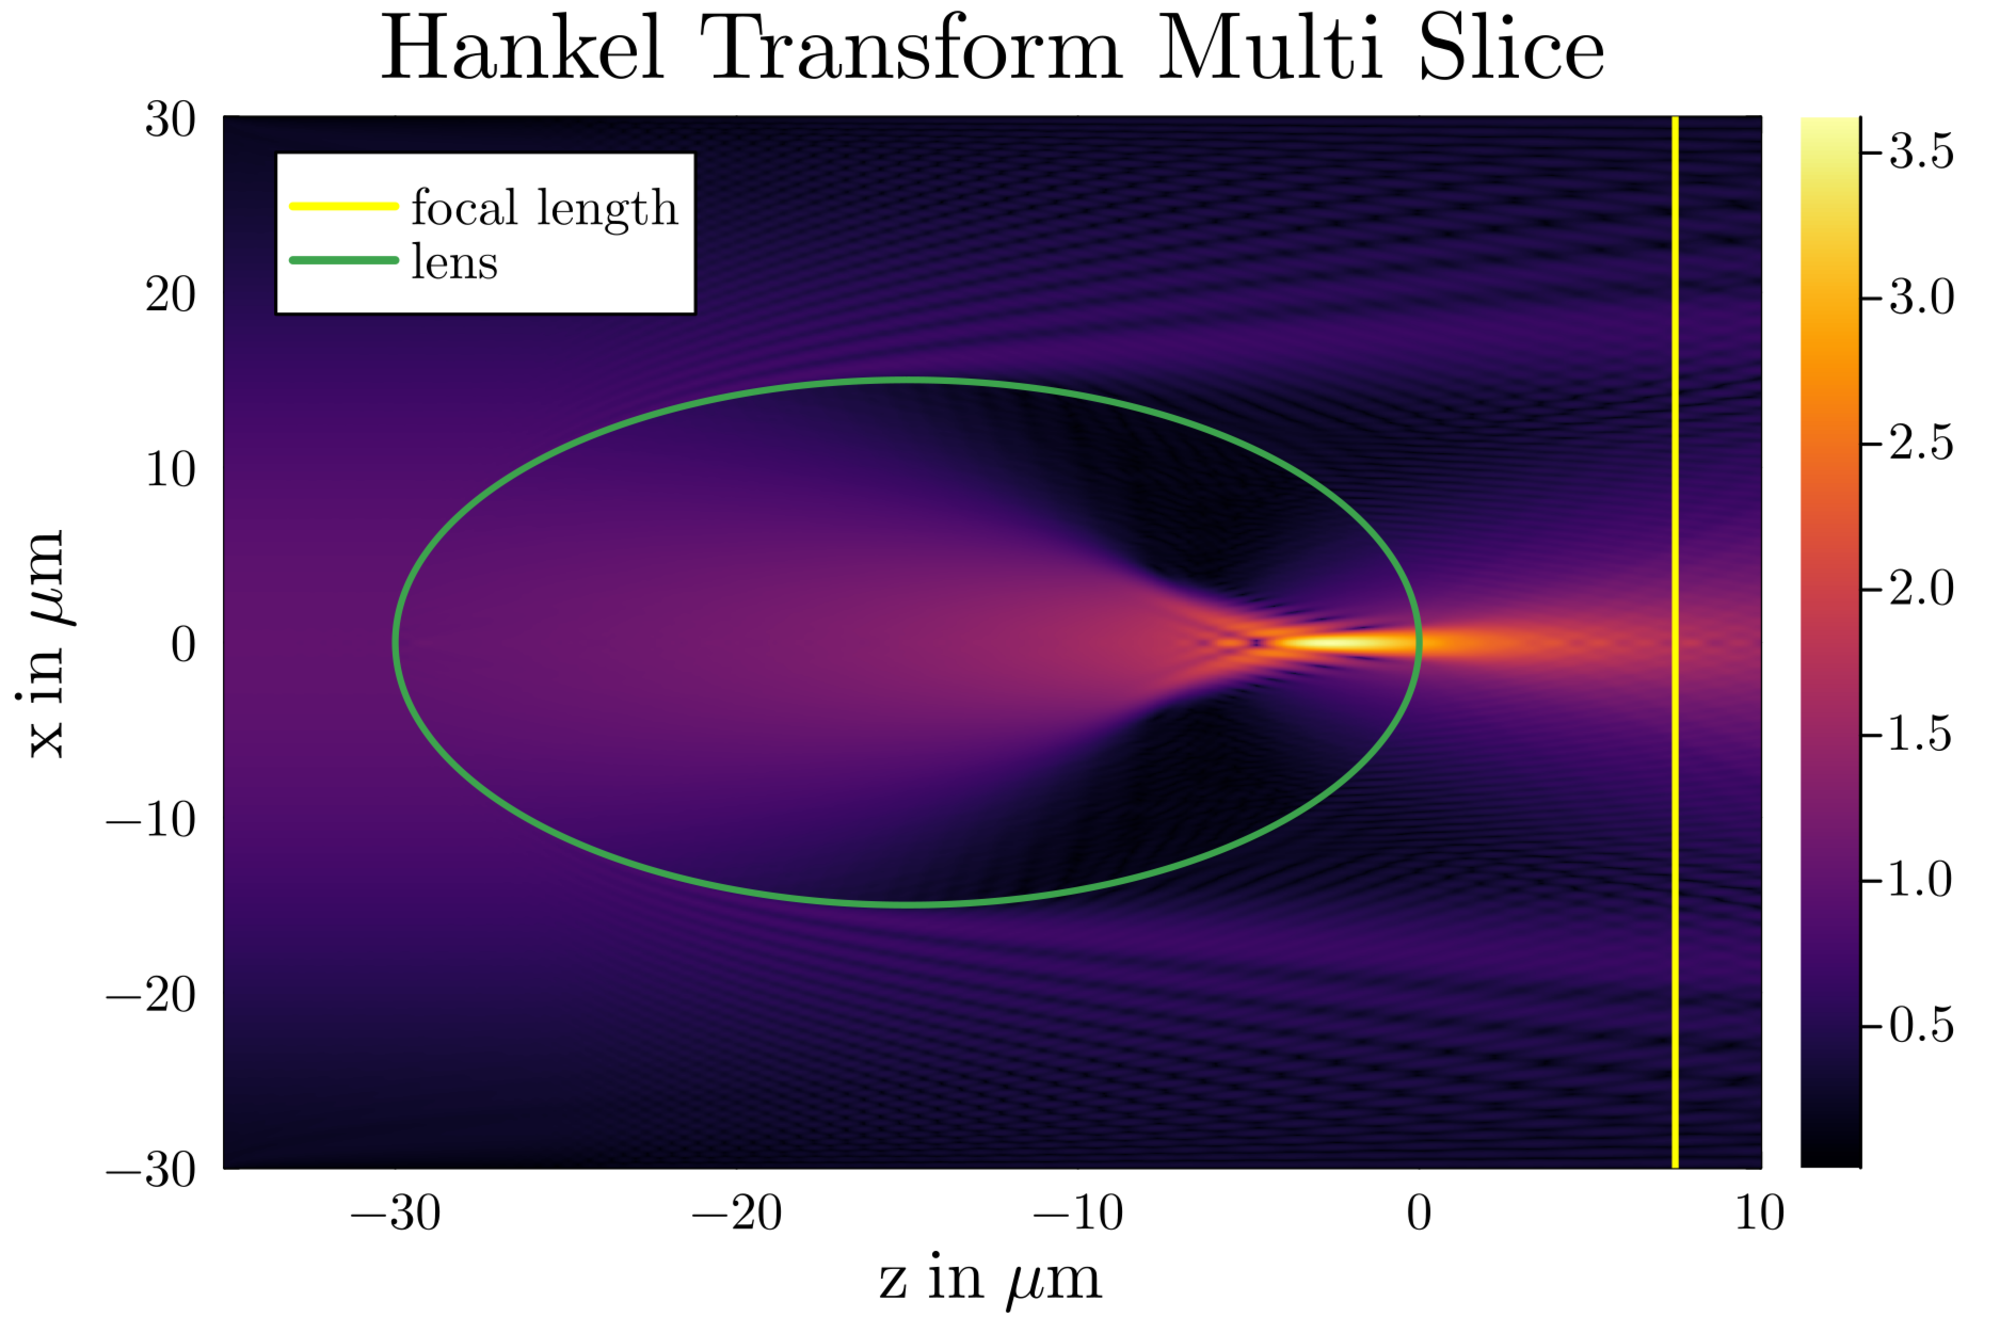
\includegraphics[width=\textwidth]{../figures/Hankel_normal.svg.png} 
    \end{subfigure}%
    \begin{subfigure}[]{0.5\textwidth}
        \centering
        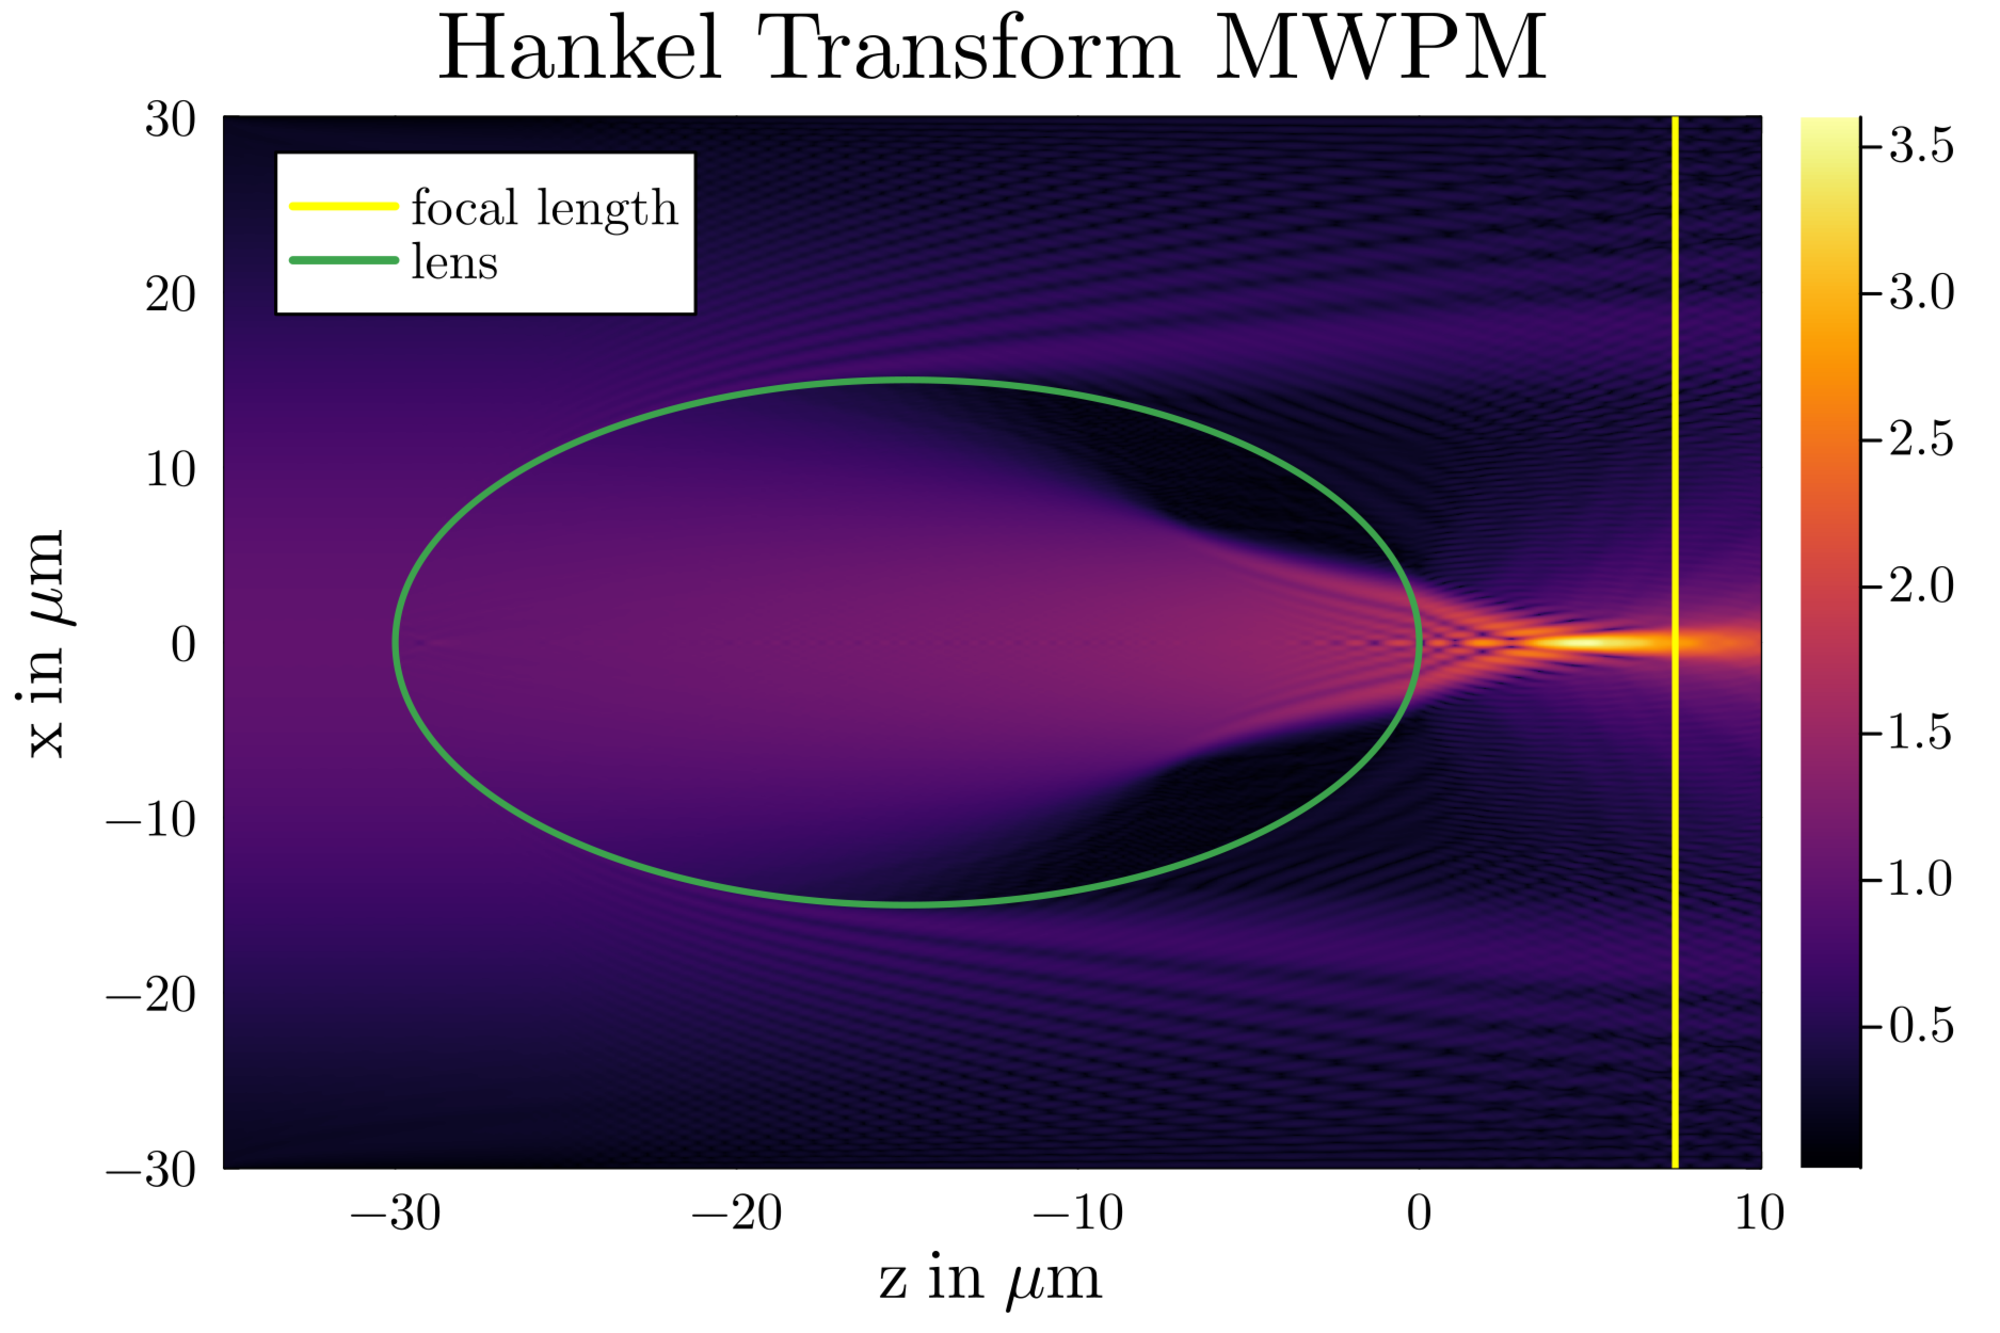
\includegraphics[width=\textwidth]{../figures/Hankel_MWPM.svg.png} 
    \end{subfigure}
    \caption{Results of the Hankel transform simulation.}
    \label{fig:}
\end{figure}
This significant decrease in computational time makes it an attractive candidate
to simulate circularly symmetric optical systems more efficiently.



\section{Conclusion}
In conclusion, we demonstrated that the multi-slice method fails to solve the homogeneous Helmholtz equation, leading to significant deviations from the geometrically derived focal length in the case of a thick lens. Similarly, the Hankel transform-based method is subject to the same physical limitations and encounters the same issue. 
However, the modified wave propagation method successfully reproduces the correct focal length for the thick lens and shows strong agreement with the results obtained from rigorous Maxwell solvers reported in the literature.

\printbibliography

\end{document}


